\subsection{Text conditioning in Diffusion Models}
\begin{frame}[allowframebreaks]{Text conditioning in Diffusion Models}
    \textbf{Text conditioning in Diffusion Models} enhances the generation of images by incorporating textual descriptions, allowing for more controlled and context-aware image synthesis.

    \begin{itemize}
        \item \textbf{Diffusion Models:} These models generate images by iteratively refining noise into coherent images, enabling high-quality synthesis.
        \item \textbf{Text Conditioning:} Uses text embeddings to guide the diffusion process, ensuring that the generated images align with specific textual descriptions.
        \item \textbf{Applications:} Image synthesis, style transfer, and content-aware editing based on textual prompts.
    \end{itemize}
\framebreak
    \begin{figure}
        \centering
        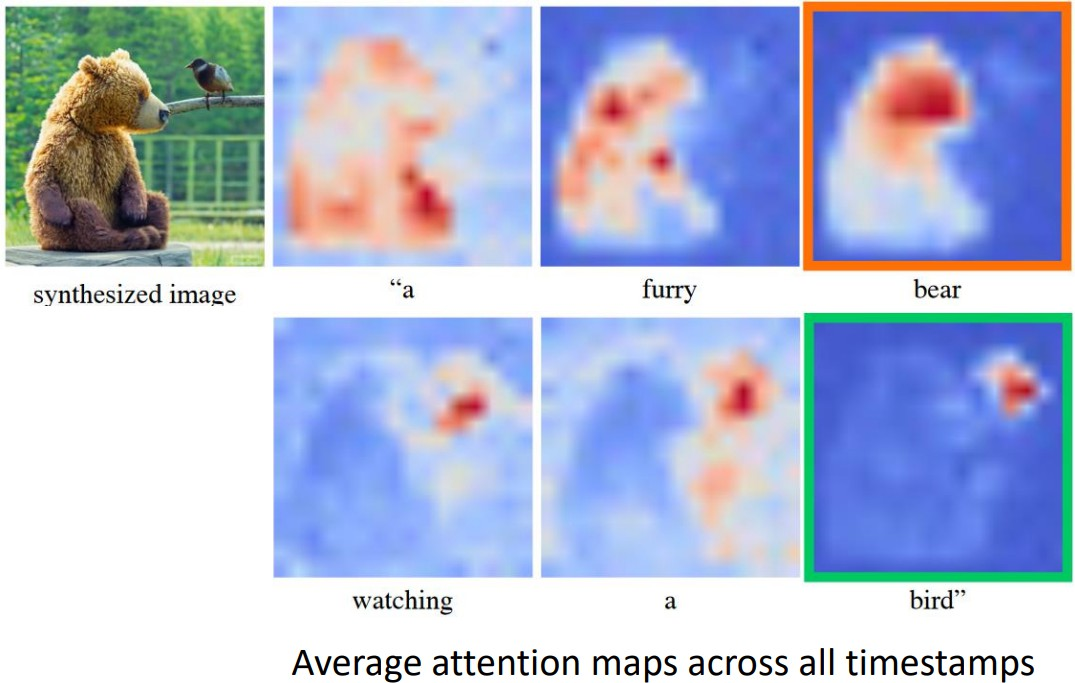
\includegraphics[width=1\textwidth,height=0.8\textheight,keepaspectratio]{images/video/slide_71_1_img.jpg}
    \end{figure}
    {\footnotesize{[Prompt-to-Prompt Image Editing with Cross Attention Control, Hertz and Mokady et al., ICRL 2022]}}
\framebreak
    \begin{figure}
        \centering
        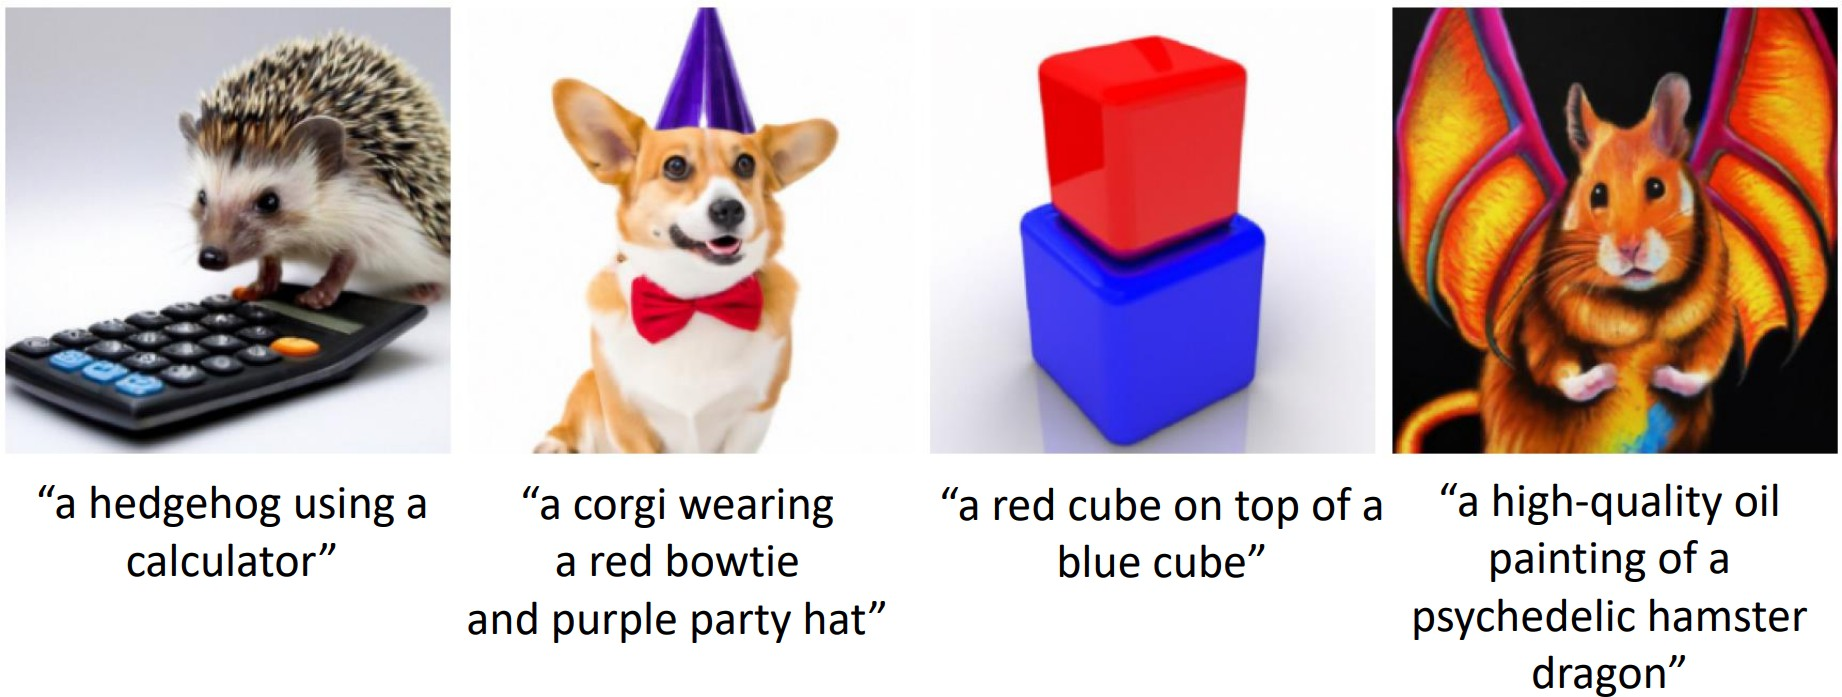
\includegraphics[width=1\textwidth,height=0.9\textheight,keepaspectratio]{images/video/slide_72_1_img.jpg}
    \end{figure}
\end{frame}